\chapter{Diskussion}
Es wurden mit verschiedenen Volumenleitermodellen, ausgehend von
vorgegebenen Dipolen im Hirnvolumen des Fötus, die resultierenden
Magnetfelder simuliert. Die Magnetfeldvektoren der Modelle wurden mit
denen von Referenzmodellen verglichen und deren Abweichungen wurden in
\textit{RDM} und Amplitudenfaktoren (\textit{MAG}) umgerechnet. Um die
Auswirkungen der Modellunterschiede auf das inverse Problem zu
untersuchen, wurden die Magnetfeldvektoren des Referenzmodells
(BEM-Modell 0 in \tablename~\ref{seq:refTable0}) für
Quellenrekonstruktionen verwendet. Die Güte der Rekonstruktionen wurde
über die Winkelabweichungen der rekonstruierten Dipole von den
vorgegebenen Dipolen und über die Faktoren der entsprechenden
Dipolstärken bestimmt.

Im Allgemeinen ensprechen die Verläufe der Ergebnisse in Abhängigkeit
von Diskretisierung, Segmentierung und Schichtdicke der Vernix caseosa
den Erwartungen mit Ausnahme der Abhängigkeit der Ergebnisse bei
Verwendung der Kopfsegmentierung von der Diskretisierung. Die
Ergebnisse der Lösung des direkten Problems korrelieren mit denen der
Lösung des inversen Problems.

Die RDM- und Amplitudenfaktorergebnisse und deren Standardabweichungen
für die Vorwärtssimulationen zeigen, dass es eine deutliche
Qualitätseinbuße bei der Verwendung der Segmentierung des Fötuskopfes
anstelle der Segmentierung des gesamten Fötus gibt. Dies spiegeln auch
die Winkelabweichungen und Amplitudenfaktoren der
Rekonstruktionsergebnisse wieder.

Beim Vergleich der verschiedenen Vernixschichtdicken fällt auf, dass
eine Reduktion der Vernixschichtdicke um 1mm bzw. $\frac{1}{4}$ genauso
wie eine Reduktion um 2mm bzw. $\frac{1}{2}$ , kaum messbare
Veränderungen in der Topologie und Amplitude der resultierenden
magnetischen Felder verursacht. Auch die Rekonstruktion von Dipolen
wurde dadurch nicht bedeutend beeinträchtigt, da die
Orientierungsabweichungen kleiner als 1° waren und die Dipolstärken mit
einem maximalen mittleren Faktor von 1.003 zu den definierten Dipolen,
sehr gut rekonstruiert wurden. Eine Veränderung der Schichtdicke der
Vernix caseoso um wenige Millimeter ist also bei der BEM-Modellierung
vom Fötus ohne maßgebliche Beeinträchtigung der Quellenrekonstruktion
möglich.

Bei klinischen Fragestellungen ist insbesondere die Genauigkeit der
räumlichen Lokalisierung der Quellen von großer Bedeutung \cite{a2},
daher wird hier die Bewertung der Lokalisierung durch den
Orientierungsfehler in \figurename~\ref{seq:refIllustration7} explizit
dargestellt.



\begin{center}
\begin{minipage}{17cm}


 [Warning: Image ignored] % Unhandled or unsupported graphics:
%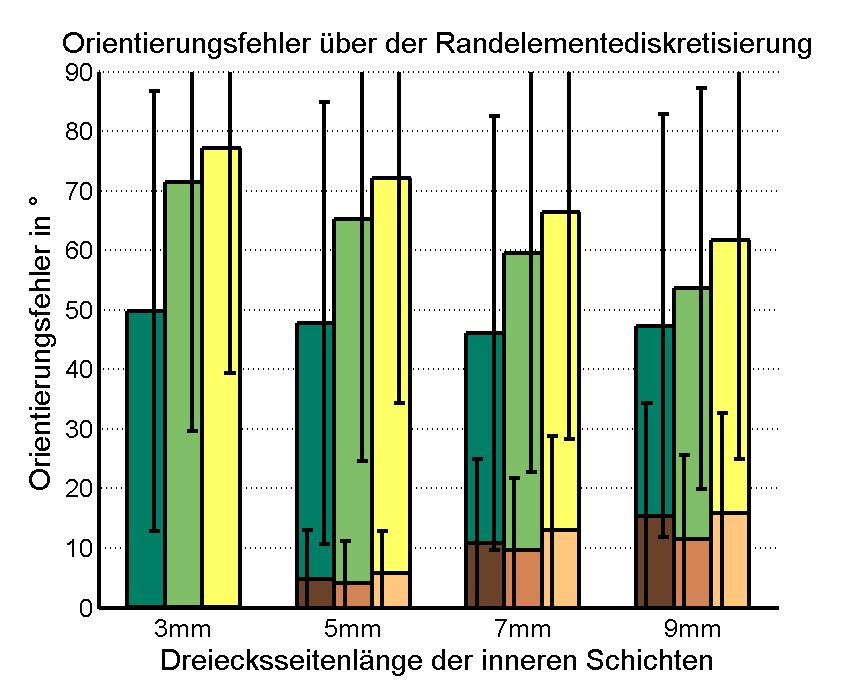
\includegraphics[width=13.723cm,height=11.289cm]{BA-img/BA-img24.eps}
\begin{center}
\tablehead{}
\begin{supertabular}{|m{8.3cm}|m{8.3cm}|}
\hline
Ausgehend von der Segmentierung des Fötus &
Ausgehend von der Segmentierung des Fötuskopfes\\\hline
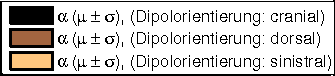
\includegraphics[width=8.304cm,height=1.884cm]{BA-img/BA-img25.png} &
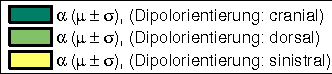
\includegraphics[width=8.304cm,height=1.85cm]{BA-img/BA-img26.png}\\\hline
\end{supertabular}
\end{center}
\captionof{figure}[Darstellung der Mittelwerte der Orientierungsfehler
und deren Standardabweichungen in ° auf der Ordinatenachse in
Abhängigkeit von der Dreiecksseitenlänge der inneren Schichten auf der
Abszissenachse]{Darstellung der Mittelwerte der Orientierungsfehler und
deren Standardabweichungen in ° auf der Ordinatenachse in Abhängigkeit
von der Dreiecksseitenlänge der inneren Schichten auf der
Abszissenachse}
\label{seq:refIllustration7}
\end{minipage}
\end{center}
Bei den BEM-Modellen, welche von der Segmentierung des Fötus erstellt
wurden, hat die Randelementediskretisierung einen direkten Einfluss auf
die Lösung in beiden Richtungen. Das heißt, größere
Dreiecksseitenlängen in den BEM-Schichten haben größere Abweichungen
der RDM- und MAG-Ergebnisse von den Idealwerten in der Vorwärtslösung
und gleichzeitig größere Fehler der rekonstruierten Dipolorientierungen
(\figurename~\ref{seq:refIllustration7}) und Dipolstärken zur Folge.
Beispielsweise verdoppeln sich die Differenzen dieser 4 Kenngrößen von
den minimalen Fehlern bei der Verwendung einer Dreiecksseitenlänge von
7mm anstelle von 5mm in den inneren Schichten. Diese Verdoppelung ist
in etwa proportional der Anzahl der verwendeten Dreiecke bzw. Knoten in
den BEM-Modellen. Die Schlussfolgerung ist, dass hier bei der
Modellierung des gesamten Fötus keine Überdiskretisierung gemacht
wurde, da andernfalls numerische Fehler eine Verschlechterung der
Lösung des inversen Problems bei zu feiner Diskretisierung verursachen.

Anders ist es bei der Verwendung der Segmentierung des Fötuskopfes, hier
bewirken größere Dreiecksseitenlängen größere Abweichungen in der
Vorwärtslösung aber kleinere Fehler bei der Lösung des inversen
Problems (\figurename~\ref{seq:refIllustration7}). Die BEM-Schichten,
welche den Fötuskopf und dessen Vernix caseosa modellieren, haben eine
sphärische Geometrie, die aufgrund der begrenzten Detailerkennbarkeit
in den Ultraschallbildern nur grob geschätzt ist. Bei dieser Geometrie
wird eine örtliche Überabtastung bei der Diskretisierung durchgeführt,
welche bei der Vorwärtslösung in diesem Fall keine negativen
Auswirkungen hat aber bei der Lösung des inversen Problems numerische
Fehler verursacht.

Wenn ein BEM-Modell, dessen innere Schicht den Fötuskopf modelliert
(BEM-Modell 4), als Referenz für diese Art von Modell verwendet wird,
dann sind die Abweichungen der Felder von Dipolen in diesen Modellen in
Abhängigkeit von der Randelementediskretisierung größer als die der
Felder von Modellen, in denen die innere Schicht den gesamten Fötus
modelliert (BEM-Modell 0 als Referenz).Dies lässt sich auf die
Geometrie der BEM-Schicht des Fötus zurückführen, die aufgrund der
begrenzten Auflösung und des schwachen Kontrastes in den
Ultraschallbildern eher konvex und geschlossen ist. Die Kopfmodelle
haben eine wesentlich kleinere Oberfläche und daher haben die
Dreiecksseitenlängen größere Einflüsse auf die Geometrie und damit auf
die magnetischen Feldvektoren.

Bei den BEM-Modellen, deren Grundlage die Segmentierung des Fötuskopfes
ist, ist eine Abhängigkeit der untersuchten Kenngrößen
(\textit{RDM},\textit{ MAG},\textit{ a} und $\alpha $) für die
Bewertung der Lösung des direkten und inversen Problems, von der
Dipolorientierung erkennbar. Dies ist ebenfalls auf die Geometrie des
Fötus zurückzuführen, welche eine stärkere Anisotropie als die
sphärische Geometrie des Fötuskopfes aufweist.

Ein guter Kompromiss ist ein Modell dessen innere Schichten den gesamten
Fötus modellieren und eine Auflösung von ca. 5mm haben, vgl. BEM-Modell
1, wobei die Vernixschichtdicke wenige Millimeter von der realen
abweichen kann. Eine Dreiecksseitenlänge von 16mm beim Abdomen und 5mm
in den inneren Schichten ist ausreichend, um Orientierungsabweichungen
von ca. 5° und Amplitudenfaktoren von ca. 0.97 zu erreichen.

In einer weiteren Studie könnten die Auswirkungen von Rauschen in den
simulierten Feldern auf die Quellenrekonstruktion untersucht werden. Es
könnte zusätzlich eine vergleichbare Studie unter Berücksichtigung des
fötalen EEG (fEEG) durchgeführt werden, sowohl kombiniert mit fMEG als
auch separat. Der Einfluss von Dipoltiefe, betrachteter Gehirnregion
und quasisphärischer Korrektur auf die Genauigkeit der Lösung des
direkten und inversen Problems bei dem MEG des Fötus sollte noch
quantifiziert werden, so wie es bereits beim MEG und EEG des
Erwachsenen gemacht wurde \cite{a2}.
